% sections/synthesis.tex
\section{Literature synthesis}\label{sec:synthesis}

\subsection{Search, screening and classification}\label{sec:litmethods}

A systematic search following PRISMA guidelines queried Web of Science, Scopus and ScienceDirect for peer reviewed empirical studies published between 2010 and 2025, with supplementary searches of Google Scholar and NOAA repositories. Boolean strings combined MHW terminology (``marine heatwave*'', ``ocean warming''), a marine scope term, impact descriptors (effect*, response*, vulnerability), biological endpoints (mortality, growth, abundance, distribution), the taxonomic term fish*, and methodological terms (regression, model*, statistic*); eligibility extended to finfish and invertebrate fisheries species. Full search syntax is given in Online Resource 1, Table S1.

Screening proceeded in two stages. Studies entered the eligible pool if they investigated MHWs or anomalous warm water events, reported biological or ecological responses of marine or euryhaline fauna, and concerned marine or brackish systems with oceanic connectivity. From that pool (1,221 full texts assessed, 1,083 retained; Online Resource 1, Fig.~S1), studies entered the analytical subset if they also applied an explicit event based thermal framework specifying baseline climatology, statistical threshold and minimum duration \citep[or equivalent;][]{hobday2016}, used an empirical observational, experimental or modelling design with quantitative assessment, and reported numerical estimates of biological change. Seventy six studies met all criteria (Online Resource 1, Fig.~S1). Records were managed in Covidence; screening conflicts were resolved by consensus, and a modified CASP checklist was used to appraise design robustness, definition clarity and transparency.

A structured template captured metadata, study characteristics, exposure type and data product, biological responses, modelling framework, covariates, validation procedures and data availability. Response terms were mapped to sub metrics and then to five response families (Population\slash Demography, Physiology\slash Bioenergetics, Distribution\slash Range\slash Phenology, Community\slash Ecosystem, Fisheries\slash Economics) using curated regular expression rules listed in full in Online Resource 1, Table S2, so that every assignment can be inspected. Modelling frameworks were assigned to one of five classes defined by their inferential logic rather than their software: association models, which relate exposure descriptors to responses under conditional independence; structured dependence models, which explicitly parameterise temporal or spatial covariance (autoregressive and state space models, distributed lag models, and Gaussian Markov random field models fitted by INLA, VAST or sdmTMB); correlative prediction models (species distribution models and machine learning aimed at spatial prediction); experimental and quasi experimental designs; and ecosystem or end to end models. Assignment used keyword dictionaries with manual verification against the full text. Co authorship and collaboration networks were analysed in VOSviewer \citep{vaneck2010}; data handling used R \citep{rcore2024}.

\subsection{Defining exposure}\label{sec:exposure}

Across the 1,083 eligible full texts, exposure was defined to suit the question at hand rather than to a common standard (Table~\ref{tab:exposure}). Only 126 studies (11.6\%) adopted the event based \citet{hobday2016} framework, under which an MHW is a run of at least five days above a climatological percentile threshold; of these, the 76 that also modelled a biological response form the analytical subset. The remainder described ``warming events'' or ``anomalous conditions'' without thresholds (553 studies), used process specific descriptors such as acute or fluctuating warming, framed exposure as projected warming under CMIP scenarios (298 studies), or built cumulative indices such as degree days that integrate intensity and duration through a biological rather than a statistical threshold \citep[e.g.][]{brown2021}. Cold anomalies appeared as a primary exposure in eight studies.

\exposureTable

Within the analytical subset, baseline choice was the main source of inconsistency. \citet{hobday2016} recommend a 30 year climatology; the reviewed studies used 1982 to 2011, 1985 to 2015, shifting windows, or did not state a baseline. Studies relying on satellite or reanalysis products frequently inherited the provider's internal climatology without reporting it \citep[e.g.][]{abookire2022,brown2021}. Fixed baselines support attribution to anthropogenic warming but progressively classify historically extreme conditions as normal; shifting baselines track contemporary norms at the cost of obscuring the trend \citep{smith2025}. Either is defensible. What constrains synthesis is that the choice changes detected intensity and duration, so that effect sizes reported against different baselines are not on a common scale, and Section~\ref{sec:simdesign} shows the magnitude of that sensitivity for one well documented event (Online Resource 1, Table S5).

A second source of inconsistency is the aggregation of daily detection to the cadence of the biological data. Most studies summarised exposure to weekly, monthly or annual values to match surveys or catch records. Aggregation is unavoidable, but it conflates short intense pulses with longer moderate warming, and it discards the timing information that lagged responses require. The simulation measures the cost of the latter directly.

\subsection{Classifying responses}\label{sec:responses}

Biological endpoints were harmonised by mapping raw terms to sub metrics and then to five families with curated regular expressions (Online Resource 1, Table S2). Population\slash Demography, which includes fishery dependent indices such as catch per unit effort (CPUE) and landings, and Physiology\slash Bioenergetics dominated; Distribution\slash Range\slash Phenology followed; Community\slash Ecosystem endpoints were less common and Fisheries\slash Economics endpoints appeared in a single study (Fig.~\ref{fig:responses}). Abundance, survival, growth and biomass were the most frequent terms.

\begin{figure}[H]\centering
\panel{a}{0.56\textwidth}{lit_cooccurrence_submetric}\hfill\panel{b}{0.42\textwidth}{lit_cooccurrence_family}\\[8pt]
\panel{c}{0.40\textwidth}{lit_wordcloud}\hfill\panel{d}{0.58\textwidth}{lit_submetric_counts}
\caption{Patterns in biological response measurement across the 76 studies. (a) Number of studies in which each pair of sub metrics was co measured; grey cells mark the diagonal. (b) The same co occurrence among the five response families. (c) Raw response terms, sized by frequency. (d) Number of studies reporting each sub metric, by response family.}
\label{fig:responses}
\end{figure}

Co measurement patterns are informative. Population\slash Demography pairs most often with Physiology\slash Bioenergetics, where organism level stress is measured together with demographic outcomes, and almost as often with Distribution\slash Range\slash Phenology, reflecting designs that track abundance alongside range or habitat change (Fig.~\ref{fig:responses}b). The three abundance proxies, however, almost never appear together: CPUE comes from fishery dependent records, abundance and density from surveys, and biomass from ecosystem model output. Each proxy follows its data infrastructure, and studies rarely triangulate across them. For a fisheries audience this is the most consequential pattern in the response data, because CPUE based impact estimates and survey based estimates answer different questions about the same event and are rarely reconciled.

Publication volume grew from 2016, peaked in 2021 with 18 studies and has remained at 11 to 13 per year since; the growth was carried by population and physiology studies, while community and economic endpoints stayed flat (Online Resource 1, Fig.~S2 and accompanying text).

\subsection{Where the work is done}\label{sec:geography}

Research effort is concentrated. The United States and Australia contributed roughly 47 of the 76 studies; the Northeast Pacific event alone accounts for 30, and Australian waters for 14 (Fig.~\ref{fig:map}). The tropical Pacific, South Atlantic, Bay of Bengal and much of the Indian Ocean are nearly absent despite documented MHW activity. Institutions studied events in their own regional waters, so the literature reflects the location of observing infrastructure as much as the ecological significance of events. Co authorship networks confirm the pattern: a small number of institutional hubs anchor dense regional clusters, and connectivity beyond them is sparse (Online Resource 1, Fig.~S3 and accompanying text). Methodological innovation therefore diffuses unevenly, and the regions most exposed to future MHWs are the least equipped to assess them.

\begin{figure}[H]\centering
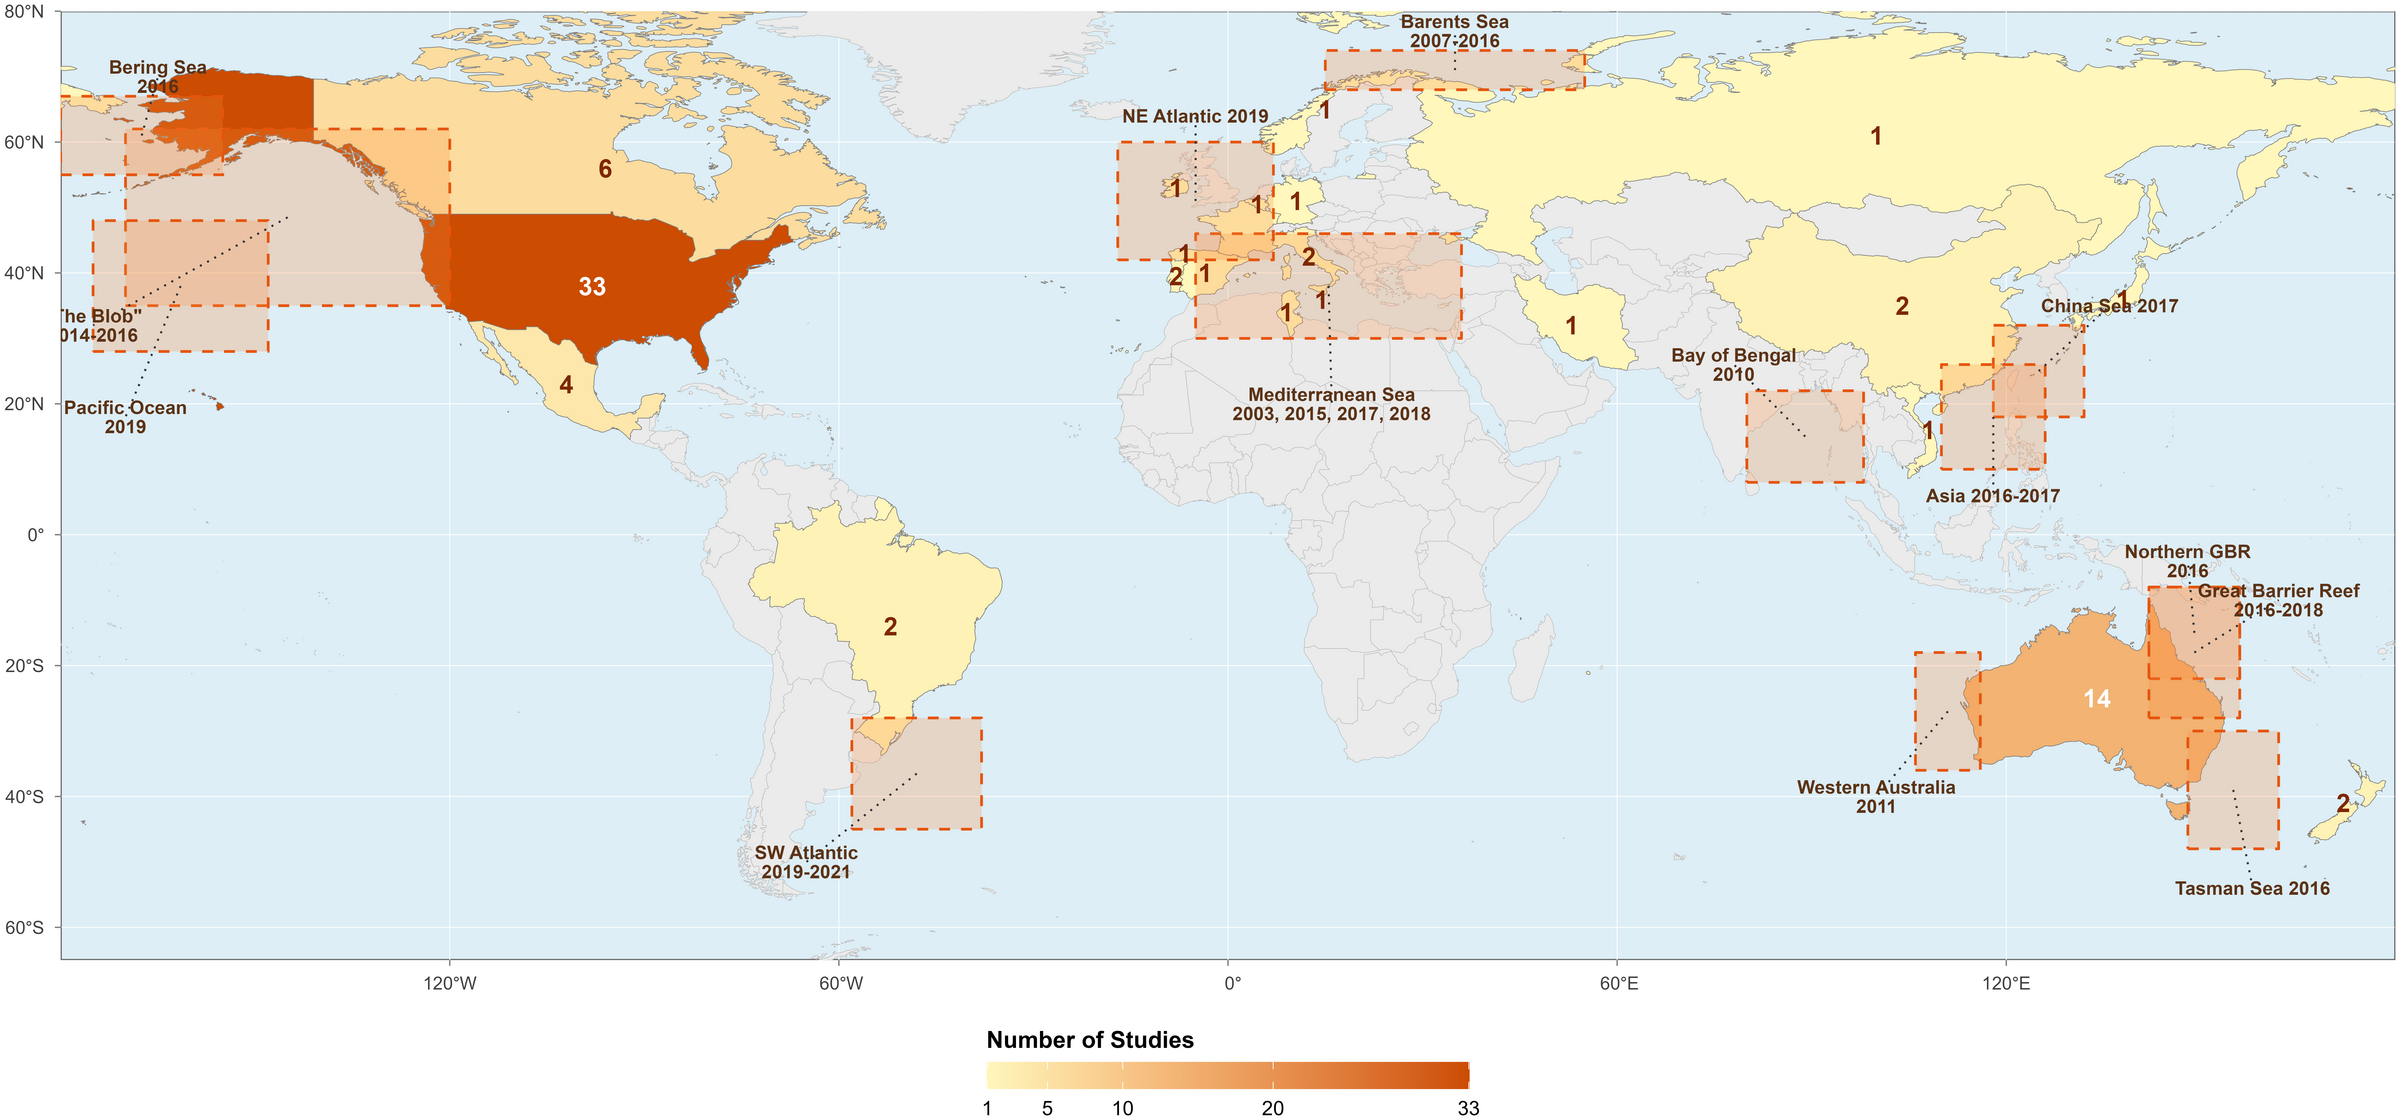
\includegraphics[width=\textwidth]{lit_map}
\caption{Geographic concentration of the evidence base. Country shading and the printed numbers give the number of studies contributed by institutions based in each country; dashed rectangles give the approximate extents of the named marine heatwave events, with their years, to which the studies are linked.}
\label{fig:map}
\end{figure}

\subsection{Modelling frameworks in practice}\label{sec:frameworks}

Table~\ref{tab:frameworks} summarises the framework classes, the inferential question each answers, the dependence structure each represents, the data each requires and the R implementations used in the simulation. The classification is by inferential logic: a GAM used to map habitat suitability is a correlative prediction model, while the same GAM used to estimate a lagged exposure effect is an association model.

\begin{table}[H]
\centering
\caption{Framework classes used to link marine heatwave exposure to biological responses in the 76 reviewed studies. The dependence column states what each class treats as estimable structure; the data column states the minimum data configuration under which the class is identifiable. Software columns name the R implementations used in this review's simulation and widely used alternatives. GLM, generalised linear model; GLMM, generalised linear mixed model; GAM, generalised additive model; DLNM, distributed lag non linear model; GMRF, Gaussian Markov random field; SPDE, stochastic partial differential equation; SDM, species distribution model; BRT, boosted regression trees.}
\label{tab:frameworks}
\small
\setlength{\tabcolsep}{4pt}\begin{tabular}{p{2.5cm}p{3.3cm}p{3.0cm}p{3.2cm}p{2.6cm}}
\toprule
Class & Inferential question & Dependence represented & Minimum data & R implementations \\
\midrule
Association (GLM, GLMM, GAM) & Is exposure related to the response, and how strongly? & None (GLM) or exchangeable random effects for sites or years (GLMM, GAM) & Response and exposure at matched cadence; any sample size the family supports & MASS, lme4, glmmTMB, mgcv \\
\addlinespace
Structured dependence: temporal (AR, state space, DLNM) & When does the response occur relative to exposure, and over how long? & Autocorrelation and lag structure in time & Response series long enough to resolve the lag; at least 3 to 5 cycles of the longest lag & dlnm, MARSS, KFAS \\
\addlinespace
Structured dependence: spatial and spatiotemporal (GMRF\slash SPDE) & How does the effect vary in space, and how much residual spatial structure remains? & Spatially correlated latent field, optionally evolving in time & Observations at enough distinct locations to estimate a range parameter; gridded or irregular & sdmTMB, INLA, VAST \\
\addlinespace
Correlative prediction (SDM, BRT, random forest) & Where will the species be, given covariates? & None explicit; captured implicitly through covariates & Occurrence or abundance with covariate fields; cross-validation blocked in space or time & dismo, ranger, gbm \\
\addlinespace
Experimental and quasi experimental & Does exposure cause the response? & Controlled by design (randomisation, before after control impact) & Replicated treatments or a credible control series & Standard linear and mixed models \\
\addlinespace
Ecosystem and end to end (Ecopath, Ecosim, EcoTroph) & How do impacts propagate through the food web? & Trophic linkages and mass balance & Diet matrices, production and consumption ratios, biomass time series & Rpath \\
\bottomrule
\end{tabular}
\end{table}

\paragraph{Association models dominate by default.}
Generalised linear and mixed models link event metrics to responses using fishery dependent and survey data aggregated to weekly or monthly resolution \citep{brown2021,caputi2016,hart2018,mann2021}. They handle zero inflation, overdispersion and nesting without heavy parameterisation, and they are accessible without specialised training; their prevalence reflects the data and the analysts available rather than a judgement about inferential fit. Generalised additive models are comparatively underused despite their suitability for non linear and seasonal responses \citep{becker2019,fredston2023}. Where they have been applied they revealed structure that parametric specifications miss: smooths over lagged intensity exposed delayed effects \citep{abookire2022,blixt2025}, tensor products captured depth by temperature interactions \citep{becker2019}, and derivative summaries flagged candidate regime shifts \citep{blixt2025}. Diagnostics appropriate to smooth models, such as basis dimension checks and concurvity screening, are rarely reported in parametric studies, so undetected non linearity in GLM based estimates cannot be ruled out. Validation in this class is usually limited to residual checks and information criteria; blocked cross-validation and bootstrap uncertainty appear in a minority \citep{benedetticecchi2024,brown2021,gomes2023}.

\paragraph{Structured dependence models are rare and clustered.}
Models that parameterise temporal or spatial covariance can estimate lagged responses, separate cumulative from pulse exposure and map spatially varying effects. In the subset they appear in fewer than 10\% of studies and almost exclusively in intensively monitored systems. Temporal applications include autoregressive and state space models for humpback whale demography \citep{gabriele2022} and distributed lag structures for euphausiid size \citep{robertson2020}. Spatiotemporal applications fit GMRFs through the SPDE approximation: \citet{evans2023} used INLA to show that euphausiid biomass off Vancouver Island peaked during the 2014 to 2016 event with a Pacific Decadal Oscillation signal invisible in aggregated data; \citet{chasco2022} used VAST, which represents the spatial field as a GMRF in the same way as sdmTMB \citep{thorson2019,anderson2022}, to show that market squid expanded their range only in heatwave years; and \citet{lacheheb2024} used geographically and temporally weighted regression to map where moderate events raised New Zealand catches and extreme events lowered them. The validation practices in these studies, which include rolling origin forecasts and spatial or temporal block cross-validation, are not intrinsic to the model class; they are recommended for any model fitted to autocorrelated data \citep{roberts2017} and are simply more often followed by analysts who have already engaged with dependence. The concentration of these methods in a few author groups indicates that the constraint is expertise and data cadence rather than any lack of relevance.

\paragraph{Correlative prediction models are used for hindsight.}
Species distribution models and machine learning methods appear in MHW studies mainly for retrospective attribution: GAM based SDMs for sardine habitat availability \citep{muhling2025}, boosted regression trees for predator redistribution during four Northeast Pacific events \citep{welch2023}, and GAMs for groundfish and bluefin tuna habitat \citep{rooper2021,mcnicholas2024}. Their use for forward prediction is limited because correlative models calibrated on historical conditions assume distributional equilibrium and carry no representation of thermal limits, movement or life history \citep{welch2023,brodie2021}. Vertical redistribution during heatwaves, documented for mesopelagic fishes in the California Current \citep{iglesias2024}, is one example of a response that horizontal habitat models cannot represent.

\paragraph{Experiments supply mechanism; translation remains the problem.}
Controlled exposures quantify thermal maxima, metabolic scope, growth and survival with internal validity that observational designs cannot match \citep{anastasiadi2021,beaudreau2024,horkan2025,spencejones2025}. They show that early life exposure leaves lasting epigenetic marks, that congeneric clams differ sharply in tolerance, and that prior exposure partially buffers later events. Their authors are candid about limits: food replete, predator free conditions may not generalise \citep{spencejones2025}, and single stressor exposures are snapshots \citep{dinh2021}. The 2015 walleye pollock year class failed through interacting stressors rather than temperature alone \citep{rogers2021}, which illustrates why laboratory thresholds are better treated as mechanistic inputs to population models than as predictors of field outcomes. Quasi experimental designs that exploit natural variation in exposure, such as before after comparisons across the 2014 to 2016 event \citep{horkan2025} and a before after control impact analysis of 227 kelp forest taxa \citep{liang2024}, preserve field realism while supporting causal claims, but remain rare.

\paragraph{Ecosystem models are proofs of concept.}
Mass balance models have shown that trophic structure mediates impact: top down regulated reefs can lose most of their biomass under extreme events while bottom up systems are partly buffered \citep{artana2024}, and recovery time scales with latitude and trophic position \citep{guibourd2024}. Both studies required diet matrices, production ratios and long biomass series that exist only for intensively monitored sites. Hierarchical pooling of parameters across habitat types is the most plausible route to wider application.

\paragraph{Mixed designs.}
Since 2021 a small number of studies have combined approaches, pairing climate projections with controlled experiments \citep{moore2023} or field observation with targeted manipulation \citep{spencejones2025}. Modelling remains the dominant approach every year, experimental studies are fewer but persistent, and mixed designs have appeared only recently (Fig.~\ref{fig:approaches}). Population, distribution and community endpoints are addressed almost entirely by modelling because the relevant scales exceed what can be manipulated; physiological endpoints carry the highest experimental share.

\begin{figure}[H]\centering
\panel{a}{0.49\textwidth}{lit_approach_by_year}\hfill\panel{b}{0.49\textwidth}{lit_approach_by_family}
\caption{Study approaches in the 76 studies. (a) Annual number of publications using experimental, mixed and modelling designs, 2016 to 2025. (b) Number of studies by approach within each response family; a study contributing to several families is counted in each.}
\label{fig:approaches}
\end{figure}

\subsection{Three structural problems}\label{sec:problems}

Three problems recur across the synthesis and motivate the simulation. The measurement foundation is heterogeneous: baseline, threshold and aggregation choices are often unreported and always consequential, so reported effect sizes are not on a common scale. Framework choice follows data infrastructure and training rather than the inferential question, so lagged and non linear responses are systematically under represented in the estimates that enter the literature. And methods are reported at a level of detail that does not support re-implementation, so practice diffuses slowly from the hubs where it is developed. The first problem is a matter of reporting standards. The second is an empirical claim about estimator behaviour, and Section~\ref{sec:simulation} tests it.
